\section{Experiments}
\label{sec:evaluation}
%\todo{ALL: Preferably use \textbf{\chonk} (also ViT-e, ViT-G, ViT-g,...) everywhere in tables/figures. We can also use \chonk/14 (ViT-e/14, ViT-G/14, ViT-g/14, ViT-L/16...) if the patch-size is absolutely needed, and 22B, e, g, G, ... only if there is s shortage of space.}
% I tried to go through the whole file and remove the /patch parts. Where it wasn't clear whether they are "absolutely needed" I tried to use "track changes" for someone else to agree.

\subsection{Training details}
\label{sec:training}
\paragraph{Dataset.}
\chonk is trained on a version of JFT~\citep{sun2017revisiting}, extended to around 4B images~\citep{zhai2022scaling}.
These images have been semi-automatically annotated with a class-hierarchy of 30k labels.
Following the original Vision Transformer, we flatten the hierarchical label structure and use all the assigned labels in a multi-label classification fashion employing the sigmoid cross-entropy loss.

\paragraph{Hyperparameters.}
\chonk was trained using 256 visual tokens per image, where each token represents a $14 \times 14$ patch extracted from $224 \times 224$ sized images. 
\chonk is trained for 177k steps with batch size of 65k: approximately 3 epochs.
We use a reciprocal square-root learning rate schedule with a peak of $10^{-3}$, and linear warmup (first 10k steps) and cooldown (last 30k steps) phases. For better few-shot adaptation, we use a higher weight decay on the head ($3.0$) than body ($0.03$) for upstream training~\citep{zhai2022scaling, abnar2021exploring}. 


% Transfer
\subsection{Transfer to image classification}
Efficient transfer learning with large scale backbones is often achieved by using them as frozen feature extractors. This section presents the evaluation results of \chonk for image classification using linear probing and locked-image tuning as well as out-of-distribution transfer. Additional results for  Head2Toe transfer, few-shot transfer, and linear probing with L-BFGS can be found in \cref{app:image_classification}.

\subsubsection{Linear probing}

% We perform linear probing of the pre-logits (the representation after the pooling by MAP head) transfer to both ImageNet-1k as a standard benchmark, as well as iNaturalist~\citep{cui2018large} for benchmarking linear separability of fine-grained concepts.

We explored various ways of training a linear probe, % we defer the details to Appendix~\ref{app:linear}.
our final setup on ImageNet uses SGD with momentum for 10 epochs at 224px resolution, with mild random cropping and horizontal flipping as the only data augmentations, and no further regularizations.
% (no L2 penalty).
% Isn't it clear that there's no l2? We can add it if amigious


The results presented in \cref{tab:linear_probe_i1k} show that while the returns are diminishing, there is still a notable improvement at this scale\footnote{We repeated a subset of the experiments multiple times and the results are almost identical.}.
Furthermore, we show that linear probing of larger models like \chonk can approach or exceed performance of full fine-tuning of smaller models with high-resolution, which can be often cheaper or easier to do.


% Data from go/lb-linear
\begin{table}[ht]
    \caption{Linear evaluation on ImageNet-1k~\citep{deng2009imagenet} with varying scale. All models pre-trained on large datasets. 
    Performances of a few high-resolution fine-tuned models from are provided for reference.}
    \centering
    \setlength{\tabcolsep}{4pt}
    \resizebox{.6\columnwidth}{!}{%
    \begin{tabular}{@{} l l c c c c c @{}}
        \toprule
        Model & IN & ReaL & INv2 & ObjectNet & IN-R & IN-A \\
        \midrule
        \multicolumn{7}{l}{\textit{224px linear probe (frozen)}} \\
        \midrule
        B/32 & 80.18 & 86.00 & 69.56 & 46.03 & 75.03 & 31.2 \\
        B/16 & 84.20 & 88.79 & 75.07 & 56.01 & 82.50 & 52.67 \\
        ALIGN (360px) & 85.5 & - & - & - & - & - \\
        L/16 & 86.66 & 90.05 & 78.57 & 63.84 & 89.92 & 67.96 \\
        g/14 & 88.51 & 90.50 & 81.10 & 68.84 & 92.33 & 77.51 \\
        G/14 & 88.98 & 90.60 & 81.32 & 69.55 & 91.74 & 78.79 \\
        e/14 & 89.26 & 90.74 & 82.51 & 71.54 & \textbf{94.33} & 81.56 \\
        22B  & \textbf{89.51} & \textbf{90.94} & \textbf{83.15} & \textbf{74.30} & 94.27 & \textbf{83.80} \\
        \midrule
        \multicolumn{7}{l}{\textit{High-res fine-tuning}} \\
        \midrule
        L/16 & 88.5 & 90.4 & 80.4 & - & - & - \\
        FixNoisy-L2 & 88.5 & 90.9 & 80.8 & - & - & - \\
        ALIGN-L2 & 88.64 & - & - & - & - & - \\
        MaxViT-XL & 89.53 & - & - & - & - & - \\
        G/14 & 90.45 & 90.81 & 83.33 & 70.53 & - & - \\
        e/14 & 90.9 & 91.1 & 84.3 & 72.0 & - & - \\
        \bottomrule
    \end{tabular}
    }
    % \vspace{-5pt}
    \label{tab:linear_probe_i1k}
\end{table}

\begin{figure}[tbp]
    \centering
    % \vspace{-5pt}
    \subfigure{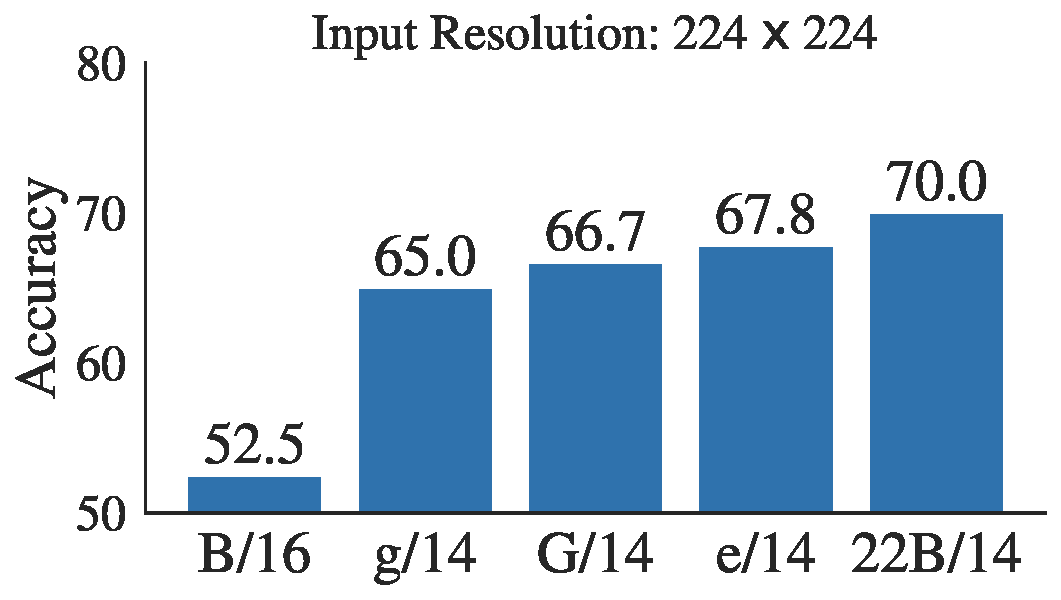
\includegraphics[width=0.35\textwidth]{figs/inat/inat-224.pdf}}
    \hspace{15pt} 
    \subfigure{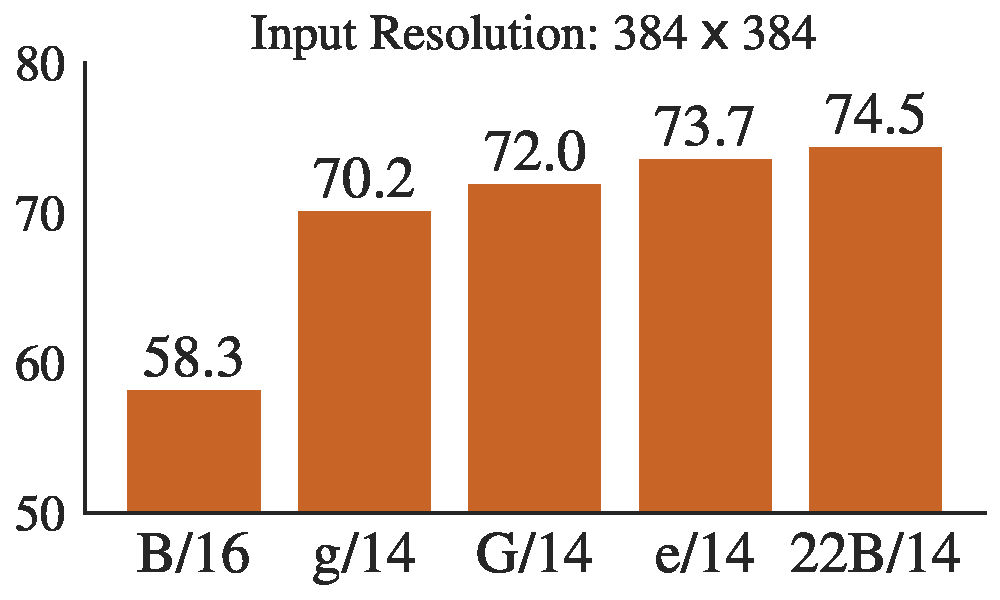
\includegraphics[width=0.35\textwidth]{figs/inat/inat-384.pdf}}
    % \vspace{-5pt}
    \caption{Linear probing on iNaturalist 2017 with different input resolutions. \chonk leads to significant accuracy improvement especially when the input size is small.}
    \label{fig:inat}
    % % \vspace{-10pt}
\end{figure}



We further test linear separability on the fine-grained classification dataset, iNaturalist 2017~\citep{cui2018large}. It has 5,089 find-grained categories, belonging to 13 super-categories. Unlike ImageNet, the image numbers in different categories are not balanced. The long-tail distribution of concepts is more challenging for classification. We compare \chonk with the other ViT variants. 
% For fair comparison, we resize the input images to a fixed size and use those models to extract features for linear classification. 
Similar to the linear probing on ImageNet, we use SGD with 0.001 starting learning rate and no weight decay to optimize the models and train for 30 epochs with cosine learning rate schedule with 3 epochs of linear warm-up. We test both $224$px and $384$px input resolutions. \cref{fig:inat} shows the results. We observe that \chonk significantly improves over the other ViT variants, especially with the standard $224$px input resolution. This suggests the large number of parameters in \chonk are useful for extracting detailed information from the images. 

\subsubsection{Zero-shot via locked-image tuning}
\label{sect::lit}
\paragraph{Experimental setup.}
Following the Locked-image Tuning (LiT)~\citep{lit} protocol, we train a text tower contrastively to match the embeddings produced by the frozen \chonk model.
With this text tower, we can easily perform zero-shot classification and zero-shot retrieval tasks.
We train a text Transformer with the same size as ViT-g~\citep{zhai2022scaling} on the English subset of the WebLI dataset~\citep{chen2022pali} for 1M steps with a 32K batch size.
The images are resized to $288$px, and the text is tokenized to 16 tokens using a SentencePiece~\citep{kudo-richardson-2018-sentencepiece} tokenizer trained on the English C4 dataset.

\paragraph{Results.}
\cref{tab:lit} shows the zero-shot transfer results of \chonk against CLIP~\citep{clip}, ALIGN~\citep{align}, BASIC~\citep{basic}, CoCa~\citep{yu2022coca}, LiT~\citep{lit} with ViT-g~\citep{zhai2022scaling} and ViT-e~\citep{chen2022pali} models. 
The bottom part of \cref{tab:lit} compares three ViT models using the LiT recipe.
On all the ImageNet test sets, \chonk{} achieves either comparable or better results. 
Notably, zero-shot results on the ObjectNet test set is highly correlated with the ViT model size. 
The largest \chonk{} sets the new SOTA on the challenging ObjectNet test set.
\Cref{app:lit} shows zero-shot classification examples on OOD images.


% leader boards:
% - INET: https://paperswithcode.com/sota/zero-shot-transfer-image-classification-on-1
% - INET-V2: https://paperswithcode.com/sota/zero-shot-transfer-image-classification-on-3
% - INET-R: https://paperswithcode.com/sota/zero-shot-transfer-image-classification-on-4
% - INET-A: https://paperswithcode.com/sota/zero-shot-transfer-image-classification-on-5
% - OBJNET: https://paperswithcode.com/sota/zero-shot-transfer-image-classification-on-6
% - INET-REAL: https://paperswithcode.com/sota/zero-shot-transfer-image-classification-on-7
\begin{table}
\centering
\caption{Zero-shot transfer results on ImageNet (variants).}
\resizebox{.5\textwidth}{!}{%
\setlength\tabcolsep{4pt} % default value: 6pt
\begin{tabular}{@{}lcccccc@{}}
 \toprule
 Model & IN & IN-v2 & IN-R & IN-A & ObjNet & ReaL \\
 \midrule
 CLIP & 76.2 & 70.1 & 88.9 & 77.2 & 72.3 & - \\
 ALIGN & 76.4 & 70.1 & 92.2 & 75.8 & 72.2 & - \\
 BASIC & 85.7 & 80.6 & 95.7 & 85.6 & 78.9 & - \\
 CoCa & 86.3 & 80.7 & 96.5 & 90.2 & 82.7 & - \\
 \midrule
 LiT-g/14 & 85.2 & 79.8 & 94.9 & 81.8 & 82.5 & 88.6 \\
 LiT-e/14 & 85.4 & 80.6 & 96.1 & 88.0 & 84.9 & 88.4 \\
 LiT-22B & 85.9 & 80.9 & 96.0 & 90.1 & 87.6 & 88.6 \\
 \bottomrule
\end{tabular}
}
\label{tab:lit}
\end{table}

\subsubsection{Out-of-distribution}
\label{subsec:robustness_ood}
% https://colab.corp.google.com/drive/1kJ1XcIWCDQKKEHf6ef9JkgONvd6pLkk3

% TODO(andstein): remove "22B/14 hot" from table & figure

\paragraph{Experimental setup.} We construct a label-map from JFT to ImageNet, and label-maps from ImageNet to different out-of-distribution datasets, namely ObjectNet~\citep{barbu2019objectnet}, ImageNet-v2~\citep{recht2019imagenet_v2} ImageNet-R~\citep{hendrycks2020imagenet_r}, and ImageNet-A~\citep{hendrycks2021imagenet_a}. ImageNet-R and ImageNet-A use the same 200 label subspace of ImageNet (constructed in such a way that misclassifications would be considered egregious~\citep{hendrycks2021imagenet_a}), while ObjectNet has 313 categories, of which we only consider the 113 ones overlapping with the ImageNet label space. For ObjectNet and ImageNet-A we do an aspect-preserving crop of the central 75\% of the image, for the other datasets we first resize them to a square format and then take a 87.5\% central crop. Image input resolution is 224px for pre-trained checkpoints and 384px, 518px, 560px for models fine-tuned on ImageNet.

\paragraph{Results.} We can confirm results from~\citep{taori2020measuring_robustness,djolonga2021robustness_transferability,kolesnikov2020big} that scaling the model increases out-of-distribution performance in line with the improvements on ImageNet. This holds true for models that have only seen JFT images, and for models fine-tuned on ImageNet. In both cases,  \chonk continues the trend of better OOD performance with larger models (\cref{fig:robustness_objectnet}, \cref{tab:robustness_ood}).
While fine-tuning boosts accuracy on both ImageNet and out-of-distribution datasets, the effective robustness~\citep{andreassen2021effective_robustness} decreases (\cref{fig:robustness_objectnet}).
Even though ImageNet accuracy saturates, we see a significant increase on ObjectNet from ViT-e/14 to \chonk.

\begin{figure}[tbp]
    \centering
    % \vspace{-5pt}
    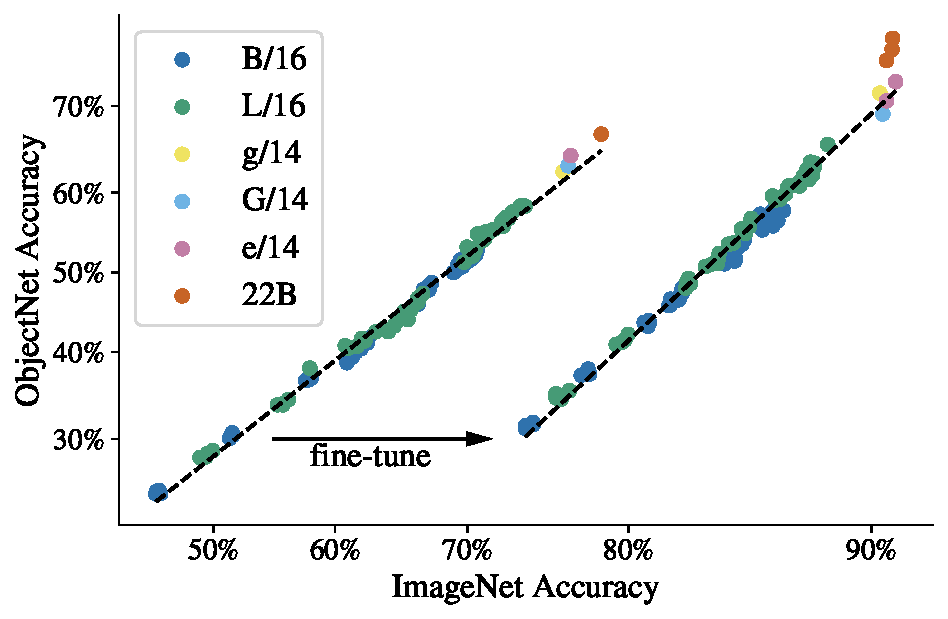
\includegraphics[width=0.6\textwidth]{figs/robustness/objectnet.pdf}
    % \vspace{-5pt}
    \caption{
        OOD classification performance. Axes are log-scaled as proposed in~\citep{taori2020measuring_robustness}. ViT-B and ViT-L are trained on subsets of varying size and varying number of steps on JFT~\citep{zhai2022scaling}. Fine-tuning boosts both ImageNet and ObjectNet performance, but the increase is more pronounced for in-domain data, which decreases effective robustness~\citep{andreassen2021effective_robustness}, visible as a rightwards shift on the plot. Same data as in \cref{tab:robustness_ood}.
    }
    \label{fig:robustness_objectnet}
    % \vspace{-15pt}
\end{figure}

\subsection{Transfer to dense prediction}
Transfer learning for dense prediction is critical especially since obtaining pixel-level labels can be costly. In this section, we investigate the quality of captured geometric and spatial information by the \chonk model (trained using image-level classification objective) on semantic segmentation and monocular depth estimation tasks.


\subsubsection{Semantic segmentation}
\paragraph{Experimental setup.}
We evaluate \chonk as a backbone in semantic segmentation on three benchmarks: ADE20K~\citep{zhou2017scene}, Pascal Context~\citep{mottaghi2014role} and Pascal VOC~\citep{everingham2010pascal}.
%Recent works have shown that plain ViT architectures can be used for dense recognition tasks~\citep{strudel2021segmenter,minderer2022simple}.
We analyze the performance in two scenarios:
first, using a limited amount of data for transfer;
second (in~\cref{app:semantic_segmentation}), comparing end-to-end fine-tuning \textit{versus} a frozen backbone with either a linear decoder~\citep{strudel2021segmenter} or UperNet~\citep{xiao2018unified}.
The number of additional parameters ($\approx1$M for linear and $\approx783$M for UperNet) is negligible compared to the size of the backbone. We use a fixed resolution ($504$px) and report single scale evaluation.

\paragraph{Results.}
We compare \chonk to the ViT-L of DeiT-III~\citep{touvron2022deit} and ViT-G of \citet{zhai2022scaling}, when only a fraction of the ADE20k semantic segmentation data is available. % during transfer.
We use the linear decoder and end-to-end fine-tuning.
From \cref{tab:semseg_fewshot}, we observe that our \chonk backbone transfers better when seeing only few segmentation masks.
For example, when fine-tuning with only 1200 images (i.e.\ $1/16$) of ADE20k training data, we reach a performance of 44.7 mIoU, an improvement of $+8.6$ mIoU over DeiT-III Large~\citep{touvron2022deit} and $+2.3$ mIoU over ViT-G~\citep{zhai2022scaling}.
When transferring with more data, the performance of ViT-G and \chonk converge.

\begin{table}[t]
    \caption{
      %\textbf
      Fewshot semantic segmentation on ADE20k, when only a fraction of the training set is used.
We report mean IoU for semantic segmentation on the validation set.
%for \chonk, ViT-L~\citep{touvron2022deit} and ViT-G~\citep{zhai2022scaling}. % the citations are already in the table
% Only a fraction
% either $1/16$, $1/8$, $1/4$, $1/2$ or $1$ (full)
% of the ADE20k training images are used. % for fine-tuning.
Transfer is done with end-to-end fine-tuning and a linear decoder, following~\citet{strudel2021segmenter}.
We average over 3 runs.
}
\centering
\small
  \setlength{\tabcolsep}{4pt}
      \resizebox{.6\textwidth}{!}{%
    \begin{tabular}{@{} l c c c c c @{}}
      \toprule
	    Fraction of ADE20k train data      & $1/16$ & $1/8$ & $1/4$ & $1/2$ & $1$ \\
      \midrule
      ViT-L~\citep{touvron2022deit} & 36.1 & 41.3 & 45.6 & 48.4 & 51.9 \\
      ViT-G~\citep{zhai2022scaling} & 42.4 & 47.0 & 50.2 & 52.4 & \textbf{55.6} \\
      \chonk (Ours) & \textbf{44.7} & \textbf{47.2} & \textbf{50.6} & \textbf{52.5} & 54.9 \\
      \bottomrule
 \end{tabular}
 }
    \label{tab:semseg_fewshot}
\end{table}



\subsubsection{Monocular depth estimation}
% In order to investigate the geometric information retained by \chonk's features, we evaluate the frozen pre-trained model on a monocular depth estimation task.
% To investigate how much geometry information is retained in the features learned by \chonk we evaluate the frozen backbone on a monocular depth estimation task.

\paragraph{Experimental setup.}
%\todo{shorten to 1 paragraph}
We largely mirror the set-up explored in \citet{ranftl2021vision} and train their Dense Prediction Transformer (DPT) on top of frozen \chonk backbone features obtained from the Waymo Open real-world driving dataset~\citep{sun2020scalability}.
Here we use only a single feature map (of the last layer) to better manage the high-dimensional ViT features.
We also explore a much simpler ``linear'' decoder as a lightweight readout.
In both cases we predict $\log(1 + \text{depth})$ obtained from sparse LiDAR as the target and use Mean Squared Error (MSE) as the decoder training loss. 
We quantify performance using standard depth estimation metrics from the literature~\citep{hermann2020self, eigen2014depth} and also report MSE. We use a resolution of $224\times224$. 
Remaining details are deferred to \Cref{app:de}.

% We use the Waymo Open real-world driving dataset~\citep{sun2020scalability}, which is composed of $1280\times1920$ resolution video frames obtained from a multi-camera system, recording videos of length $20$ seconds at $10$ frames per second (fps).
% We train a decoder on top of frozen \chonk backbone features on training set frames and evaluate it on the first 5120 validation set frames from the front facing camera, sub-sampled at 5 fps and at $224\times224$ resolution.
% We compute sparse depth maps as targets by projecting the corresponding ground truth LiDAR points to the camera frame.

% For the decoder, we largely mirror the set-up explored in \citet{ranftl2021vision} and use their Dense Prediction Transformer (DPT) with minor differences (see \Cref{app:de}).
% To better manage the high-dimensional ViT features, we use the same feature map (of the last layer) in each of the four reassemble blocks.
% We also explore a much simpler ``linear'' decoder as a lightweight readout complementary to our DPT experiments.  
% Details of its architecture are deferred to \Cref{app:de}.
% In both cases we predict $\log(1 + \text{depth})$ as the target and use Mean Squared Error (MSE) as the decoder training loss. 

% We quantify performance using the following standard depth estimation metrics from the literature~\citep{hermann2020self, eigen2014depth}, and also report the MSE loss on the validation set:
% AbsRel measures the mean absolute error between the ground truth and predicted depth relative to the ground truth, while the inlier fraction metrics ($\delta$) measure the fraction of valid pixels within a certain 
% percentage
% from ground truth.
% All metrics were measured after undoing the log transformation.


\begin{figure}[tbp]
    \centering
    \subfigure[Semantic segmentation]{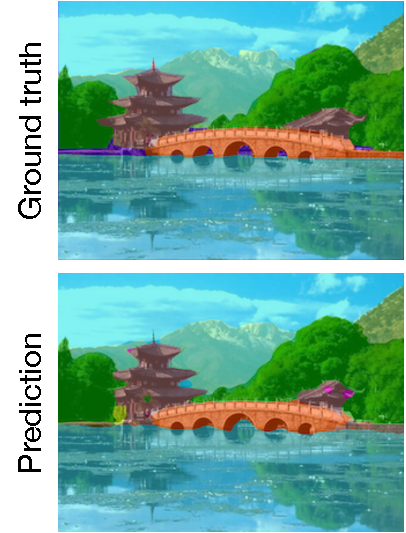
\includegraphics[width=0.315\linewidth]{figs/semseg/semantic_seg.pdf}}\quad\quad \quad\quad
    \subfigure[Depth estimation]{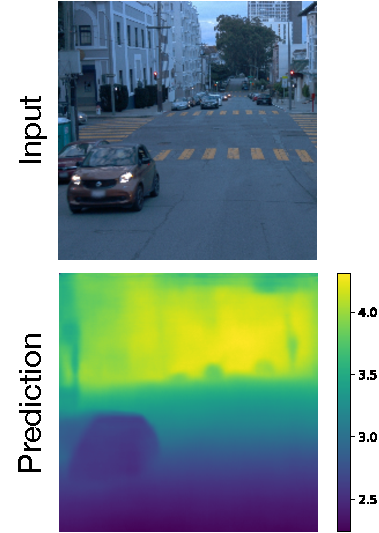
\includegraphics[width=0.2955\linewidth]{figs/depth_prediction/depth_estimation.pdf}}
    \caption{Dense prediction from frozen \chonk features.}
    \label{fig:dense_prediction}
% \vspace{-10pt}
\end{figure}

\begin{table}[t]
\caption{%\textbf
{Monocular depth estimation} from frozen ViT features using different decoders on the Waymo Open dataset.}
\centering
\small
\setlength{\tabcolsep}{4pt}
\resizebox{.55\textwidth}{!}{%
\begin{tabular}{@{} ll ccccc  @{}}
  \toprule
   & & & & \multicolumn{3}{c}{$\delta$ $\uparrow$} \\
   \cmidrule(l{2pt}r{2pt}){5-7}
    & Model      & MSE $\downarrow$ & AbsRel $\downarrow$ & $< 1.1$& $< 1.25$& $< 1.25^2$\\
  \midrule
  \multirow[c]{3}{*}{\rotatebox{90}{DPT}} & ViT-L & 0.027 & 0.121 & 0.594 & 0.871 & 0.972 \\ % xid/50851792
  & ViT-e & 0.024 & 0.112 & 0.631 & 0.888 & 0.975 \\ % xid/50851464
  & \chonk & \textbf{0.021} & \textbf{0.095} & \textbf{0.702} & \textbf{0.909} & \textbf{0.979} \\ % xid/48459029
  \midrule
  \multirow[c]{3}{*}{\rotatebox{90}{Linear}} & ViT-L & 0.060 & 0.222 & 0.304 & 0.652 & 0.926 \\ % xid/50902199
  & ViT-e & 0.053 & 0.204 & 0.332 & 0.687 & 0.938 \\ % xid/50901568
  & \chonk & \textbf{0.039} & \textbf{0.166} & \textbf{0.412} & \textbf{0.779} & \textbf{0.960} \\ % xid/50861091
  \bottomrule
\end{tabular}
}
\label{tab:depth_estimation}
% \vspace{-10pt}
\end{table}



\paragraph{Results.}
\Cref{tab:depth_estimation} summarizes our main findings.
From the top rows (DPT decoder), we observe that using \chonk features yields the best performance (across all metrics) compared to different backbones. By comparing the \chonk backbone to ViT-e (a smaller model but trained on the same data as \chonk) we find that scaling the architecture improves performance. Further, comparing the ViT-e backbone to ViT-L (a similar architecture to ViT-e but trained on less data) we find that these improvements also come from scaling the pre-training data. These findings demonstrate that both the greater model size and the greater dataset size contribute substantially to the improved performance.
%, and we find that both the greater model size and the greater dataset size contribute substantially to the improved performance from comparing ViT-L (smaller model trained on smaller data) and ViT-e (smaller model trained on the same data).
%In absolute terms, the scores obtained using \chonk appear competitive with results reported in the literature on other driving datasets.
%, indicating that we obtained good performance on Waymo Open.\todo{@gamal are there no numbers on Waymo anywhere that we can compare to roughly?}
Using the linear decoder, it can be observed again that using \chonk features yields the best performance.
% The greatly improved scores when using a DPT decoder suggest that while enough geometric information is retained in the ViT features, only some of it is available at the surface level.  
The gap between DPT and linear decoding suggests that while enough geometric information is retained in the ViT features, only some of it is available for a trivial readout.
We report qualitative results in \Cref{fig:dense_prediction} and \Cref{fig:dpt_depth_predictions_full,fig:dpt_depth_predictions_full_error} in \cref{app:de}.

% Xolab for the numbers: https://colab.corp.google.com/drive/1IjaxfaLJBNvmgLJXkicHggwyNL7uxpZ-?usp=sharing 





\subsection{Transfer to video classification}
\paragraph{Experimental setup.}
We evaluate the quality of the representations learned by \chonk by adapting the model pretrained on images for video classification.
We follow the ``factorised encoder'' architecture of~\citet{arnab2021vivit}: Our video model consists of an initial ``spatial transformer'', which encodes each frame of the video independently of each other.
Thereafter, the representation from each frame is pooled into a single token, which is then fed to a subsequent ``temporal transformer'' that models the temporal relations between the representations of each frame.

% Our choice for this architecture is motivated by the results of~\citet{arnab2021vivit}, which showed that it was an effective method for adapting image-pretrained models for video classification tasks.
% The parameters of the ``spatial transformer'' are initialized from the model pretrained on images, while the temporal transformer is trained from random initialization. Furthermore, we 
Here, we initialize the ``spatial transformer'' with the pretrained weights from ViT-22B and freeze them, as this represents a computationally efficient method of adapting large-scale models for video, and also because it allows us to effectively evaluate the representations learned by pretraining \chonk. Exhaustive experimental details are included in \cref{sec:app_video_classification}. The temporal transformer is lightweight both in terms of parameters (only 63.7M parameters compared to the 22B frozen parameters in the spatial transformer), and FLOPs as it operates on a \emph{single} token per frame.

% \todo{Exhaustive experimental details are included in \cref{sec:app_video_classification}. The temporal transformer that we learn is comparatively lightweight, consisting of 63.7 million parameters, compared to the 22 billion frozen parameters in the frozen spatial transformer.}
\paragraph{Results.}
\begin{table}[t]
    \caption{
        Video classification results.
        We evaluate the \chonk representations by freezing the backbone, and training a small transformer to aggregate frozen, per-frame representations.
        \chonk outperforms the largest previous vision backbone, ViT-e~\citep{chen2022pali} which contains 4 billion parameters and is also pretrained on JFT.
    }
    \centering{
    \resizebox{.55\textwidth}{!}{%
    \begin{tabular}{@{}lcc@{}}
        \toprule
                             & Kinetics 400 & Moments in Time \\
        \midrule
        \multicolumn{3}{l}{\textit{Frozen backbone}}                   \\
        CoCA$^*$                 &   88.0           &    47.4             \\
        ViT-e               &   86.5           &     43.6           \\  % https://xm2a.corp.google.com/experiments/49222795/workUnits/8, http://xid/51624094/3
        \chonk              &   88.0           &    44.9           \\  % https://xm2a.corp.google.com/experiments/49276809/workUnits/5, https://xm2a.corp.google.com/experiments/49597259/workUnits/3
        \midrule
        Fully finetuned SOTA &   91.1           &    49.0              \\ % https://arxiv.org/pdf/2212.03191v2.pdf, https://arxiv.org/pdf/2205.01917v2.pdf
        \bottomrule
    \end{tabular}
    }}
    \begin{adjustwidth}{110pt}{110pt}
    \begin{spacing}{0.125}{\fontsize{8pt}{5pt}\selectfont $^*$Note that CoCA uses pre-pool spatial features and higher spatial resolution for both datasets. More details in \cref{sec:app_video_classification}.}\end{spacing}
    \end{adjustwidth}
    \label{tab:results_video}
    % \vspace{-10pt}
\end{table}
\cref{tab:results_video} presents our results on video classification on the Kinetics 400~\citep{kay2017kinetics} and Moments in Time~\citep{monfort2019moments} datasets, showing that we can achieve competitive results with a frozen backbone.
We first compare to ViT-e~\citep{chen2022pali}, which has the largest previous vision backbone model consisting of 4 billion parameters, and was also trained on the JFT dataset.
We observe that our larger \chonk model improves by 1.5 points on Kinetics 400, and 1.3 points on Moments in Time. 
Our results with a frozen backbone are also competitive with CoCA~\citep{yu2022coca}, which performs a combination of contrastive and generative caption pretraining in comparison to our supervised pretraining, and uses many tokens per frame (vs.\ a single one produced by the pretrained frozen pooling) as well as a higher testing resolution.

Finally, we note that there is headroom for further improvement by full end-to-end fine-tuning. This is evidenced by the current state-of-the-art on Kinetics 400~\citep{wang2022internvideo} and Moments in Time~\citep{yu2022coca} which leverage a combination of large-scale video pretraining and full end-to-end fine-tuning on the target dataset. 
%We leave these directions for future work.




\subsection{Beyond accuracy on downstream tasks}
When studying the impact of scaling, there are important aspects to consider beyond downstream task performance. In this section, we probe \chonk's fairness, alignment with human perception, robustness, reliability, and calibration. We find that favorable characteristics emerge when increasing model size. Additional analysis on perceptual similarity and feature attribution can be found in \cref{app:perceptual_similarity} and \cref{app:feature_attribution}.


\subsubsection{Fairness}\label{sect::fairness}
Machine learning models are susceptible to unintended bias. For example, they can amplify spurious correlations in the training data~\citep{hendricks2018women,caliskan2017semantics,zhao2017men,wang2020towards} and result in error disparities~\citep{zhao2017men,buolamwini2018gender,deuschel2020uncovering}. 
Here, we identify how scaling the model size can help mitigate such issues, by evaluating the bias of \chonk  and ViT-\{L, g, G, e\} ~\citep{zhai2022scaling,chen2022pali} using demographic parity (DP) as a measure of fairness~\citep{dwork2012fairness,zafar2017fairness}.

\begin{figure}[hbt!]
    \centering
    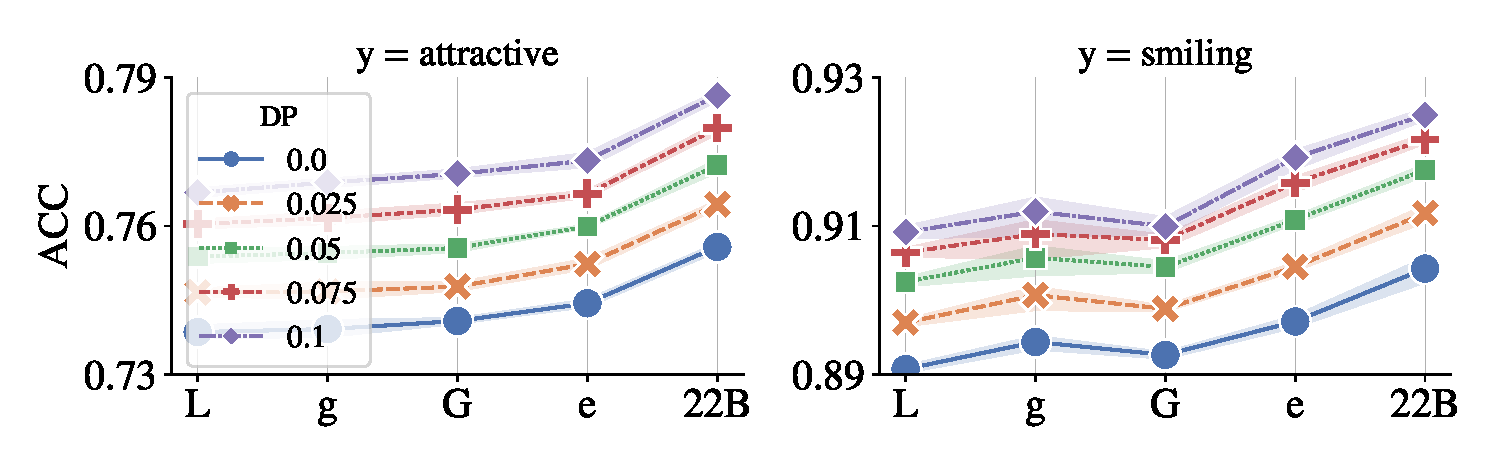
\includegraphics[width=0.7\columnwidth]{figs/fairness/perf_acc.v3.pdf}
    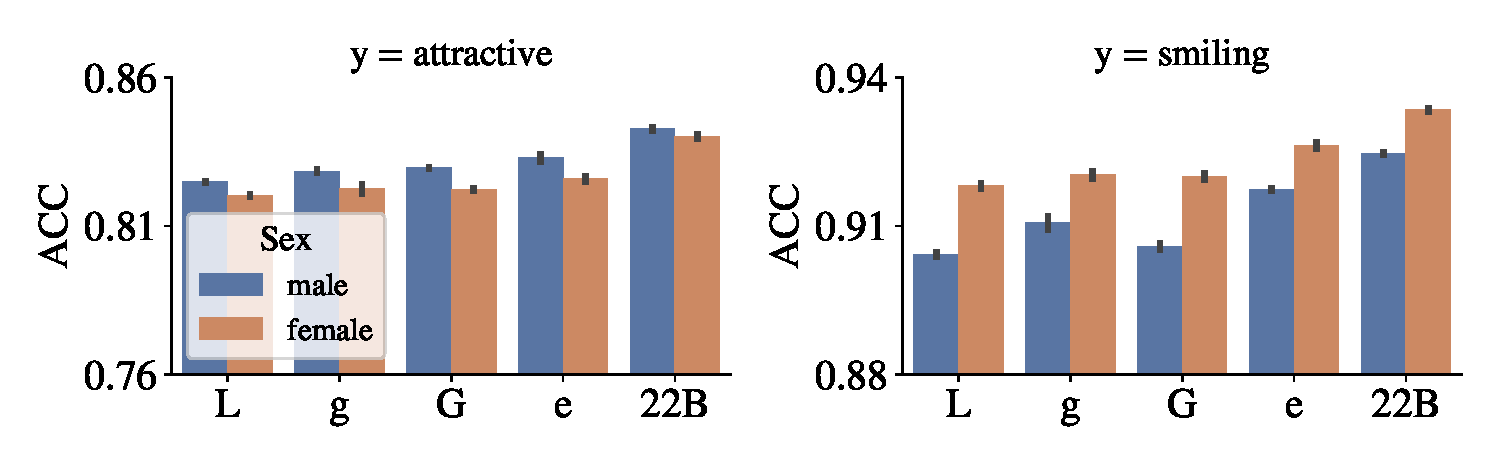
\includegraphics[width=0.7\columnwidth]{figs/fairness/all_benefit_acc_1.v3.pdf}
    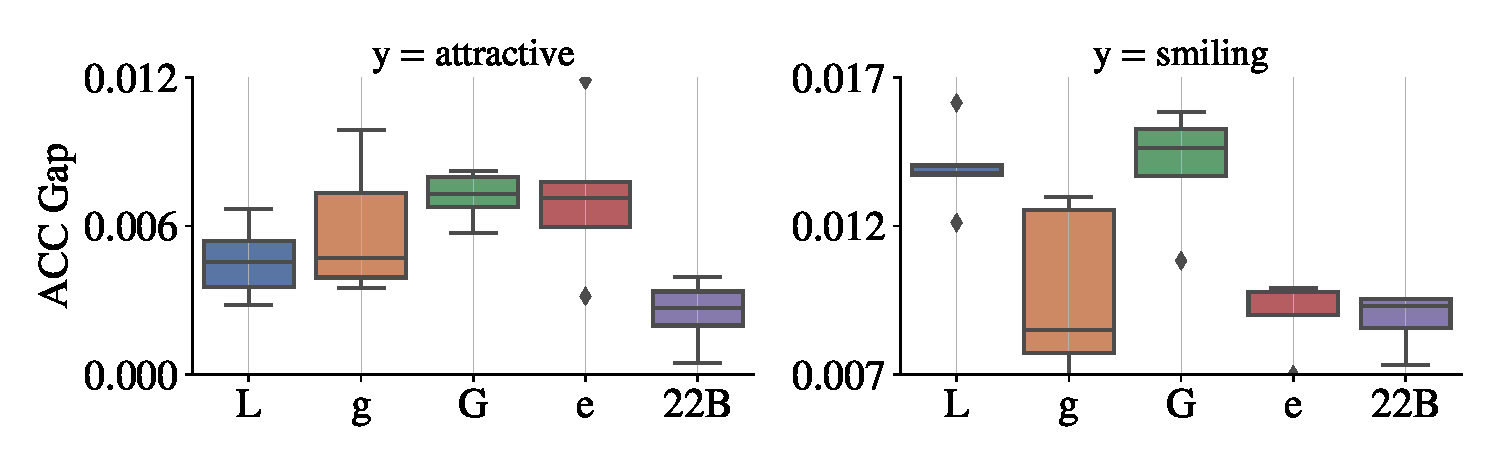
\includegraphics[width=0.7\columnwidth]{figs/fairness/parity_acc_1.v3.pdf}
    \vspace{-10pt}
    \caption{{\sc top:} Accuracy (ACC) for ViT variants \emph{after} debiasing for each DP level.  {\sc middle}: Accuracy for each subgroup in CelebA \emph{prior to} debiasing. {\sc bottom}:  $y$-axis is absolute difference in performance across the two subgroups: females and males. \chonk provides a more equitable performance, compared to smaller ViT architectures.}
    \label{fig:fairness:main}
    \vspace{-10pt}
\end{figure}

% Given a domain $\mathcal{X}$ (e.g. images) a total partitioning of $\mathcal{X}$ into subgroups $\mathcal{X}=\cup_k\mathcal{X}_k$ (e.g. based on gender or race), let $f:\mathcal{X}\to\{0, 1\}$ be a binary predictor. Then, demographic parity (DP) in $f$ with respect to $\{\mathcal{X}_k\}_k$ is defined as~\citep{dwork2012fairness,zafar2017fairness}: 
% \begin{equation}\label{eq:dp}
%     DP_f = \max_{k}\mathbb{E}[f(\textbf{x})|\textbf{x}\in\mathcal{X}_k] - \min_{k}\mathbb{E}[f(\textbf{x})|\textbf{x}\in\mathcal{X}_k].
% \end{equation}
% Extensions to the multiclass setting exist~\citep{alabdulmohsin2022}, but we focus on binary classification.


\paragraph{Experimental Setup.} We use CelebA~\citep{liu2015faceattributes} with binary gender as a sensitive attribute while the target is  ``attractive'' or ``smiling''. We emphasize that such experiments are carried out only to verify technical claims and shall by no means be interpreted as an endorsement of such vision-related tasks. We choose the latter attributes because they exhibit gender related bias as shown in \cref{fig:fairness:bias_original}.

We train a logistic regression classifier on top of the \chonk pretrained features for a total of $50$ epochs and batch size $256$, with a learning rate schedule of $0.01$ (first 25 epochs) and 0.001 (last 25 epochs).  After that, we debias using the randomized threshold optimizer (RTO) algorithm of~\citet{alabdulmohsin2021}, which was shown to be near-optimal and competitive with in-processing methods. %In RTO, we use 10K SGD steps and 1K full gradient steps, while keeping the other settings to their default values.

\paragraph{Results.}
We observe that scale by itself does not impact DP, c.f.\ \cref{fig:fairness:bias_original}. This is perhaps not surprising, as the model is trained to reconstruct a chosen target so the level of DP in accurate models is similar to that of the data itself.

However, scaling to \chonk offers benefits for fairness in other aspects. First, scale offers a more favorable tradeoff ---  performance improves with scale subject to any prescribed level of bias constraint.
This is consistent with earlier observations reported in the literature~\citep{alabdulmohsin2021}.  Second, all subgroups tend to benefit from the improvement in scale. Third, \chonk reduces disparities in performance across subgroups. 
\cref{fig:fairness:main} summarizes results for classification accuracy and \cref{app:fairness} for expected calibration error (ECE)~\citep{naeini2015obtaining,guo2017calibration} and OC-AUC~\citep{kivlichan2021measuring}.
%We use on three metrics: (1) classification accuracy (denoted ACC), (2) expected calibration error (ECE)~\citep{naeini2015obtaining,guo2017calibration}, and (3) Oracle Collaborative AUC (OC-AUC)~\citep{kivlichan2021measuring}.


\subsubsection{Human Alignment}
\label{subsec:error consistency}
%

How well do \chonk classification decisions align with human classification decisions? Using the {\tt model-vs-human} toolbox~\citep{geirhos2021partial}, we evaluate three \chonk models fine-tuned on ImageNet with different resolutions (224, 384, 560). Accross all toolbox metrics, \chonk is SOTA: \chonk-224 for highest OOD robustness (\cref{fig:model_vs_human_benchmark_a}), \chonk-384 for the closest alignment with human classification accuracies (\cref{fig:model_vs_human_benchmark_b}), and \chonk-560 for the largest error consistency (i.e.\ most human-like error patterns, \cref{fig:model_vs_human_benchmark_d}). The \chonk models have the highest ever recorded shape bias in vision models: while most models have a strong texture bias (approx.\ 20--30\% shape bias / 70--80\% texture bias)~\citep{geirhos2019imagenet}; humans are at 96\% shape / 4\% texture bias and \chonk-384 achieves a previously unseen 87\% shape bias / 13\% texture bias (\cref{fig:shape_bias}). Overall, \chonk measurably improves alignment to human visual object recognition.

\begin{figure}
    \centering
    \vspace{-5pt}
    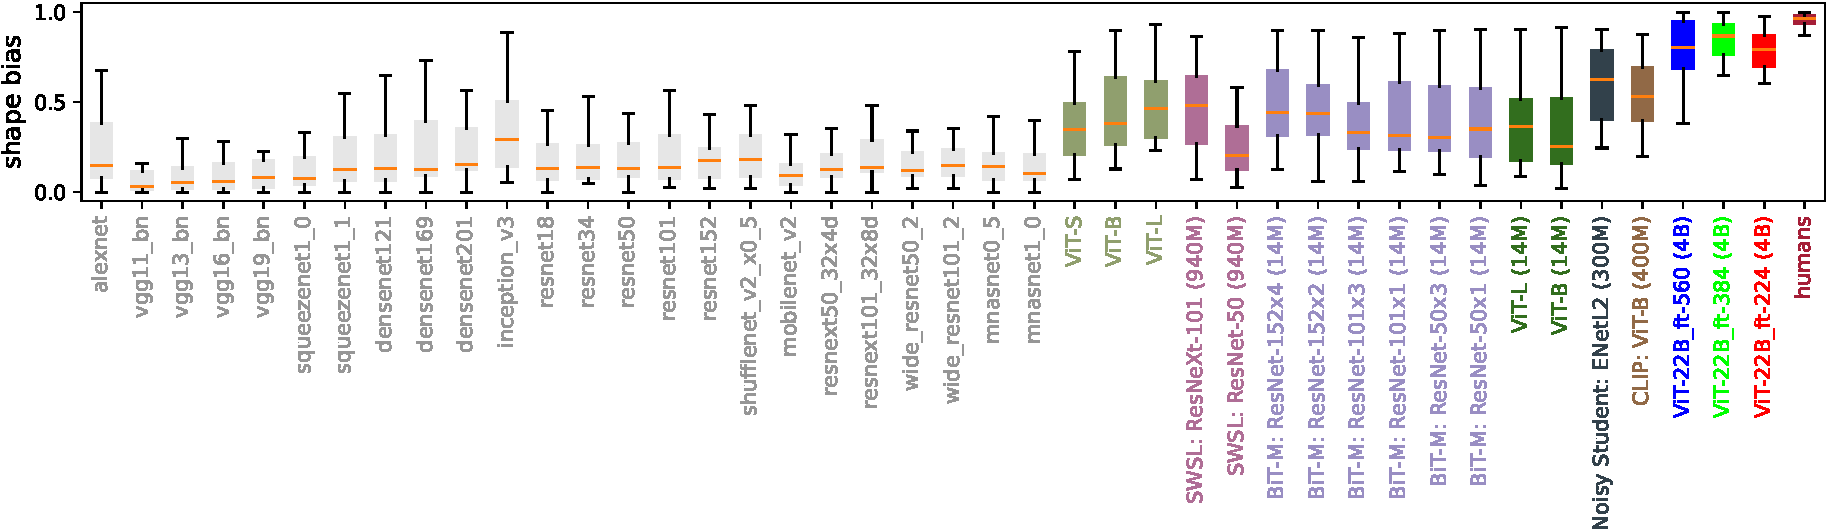
\includegraphics[width=\textwidth]{figs/human-alignment/cue-conflict_shape-bias_boxplot.pdf}
    \vspace{-0.8cm}
    \caption{Shape bias: many vision models have a low shape / high texture bias, whereas \chonk fine-tuned on ImageNet (\textcolor{red}{red}, \textcolor{green}{green}, \textcolor{blue}{blue} trained on 4B images as indicated by brackets after model names, unless trained on ImageNet only) have the highest shape bias recorded in a ML model to date, bringing them closer towards a human-like shape bias.}
    \label{fig:shape_bias}
\vspace{-10pt}
\end{figure}
%


\subsubsection{Plex - pretrained large model extensions}
\citet{tran2022plex} comprehensively evaluate the reliability of models through the lens of uncertainty, robustnes (see \cref{subsec:robustness_ood}) and adaptation (see \cref{sect::lit}).
% In this section, we focus on the first aspect of that benchmark. 
We focus here on the first aspect of that benchmark. 
To this end, we consider (1) the OOD robustness under
covariate shift with ImageNet-C~\citep{hendrycks2019benchmarking}, which we evaluate not only with the accuracy but also uncertainty metrics measuring the calibration (NLL, ECE) and the selective prediction~\citep{el2010foundations} (OC-AUC, see \cref{sect::fairness}), and (2) open-set recognition---also known as OOD detection~\citep{fort2021exploring}, which we evaluate via the AUROC and AUPRC, with Places365 as the OOD dataset~\citep{hendrycks2019scaling}; for more details, see \cref{app:plex}.

% , selective prediction~\citep{el2010foundations} 
% and label uncertainty~\citep{dusenberry2020analyzing}.

In \cref{tab:plex}, we report the performance of ViT-L and ViT-22B (both with resolution 384) fine-tuned on ImageNet. 
To put in perspective the strong gains of ViT-22B, we also show Plex-L, a ViT-L equipped with the two components advocated by \citet{tran2022plex}, viz, efficient-ensemble~\citep{wen2019batchensemble} and heteroscedastic layers~\citep{collier2021correlated}.
% to better capture model and data uncertainty respectively (Plex-L). 
We discuss the challenges and the results of the usage of those components at the 22B scale (Plex-22B) in \cref{app:plex}.

% \begin{table}[t]
%     \caption{Placeholder for PLEX~\citep{tran2022plex} results.}
% \centering
% \small
%   \setlength{\tabcolsep}{4pt}
%   \resizebox{\columnwidth}{!}{%
%     \begin{tabular}{@{} l c c c c c @{}}
%       \toprule
% 	    Evaluations      & IN-C & OOD det. & Sel.~Pred. & Lab.~Unc. \\
%       \midrule
%       ViT-L~\citep{tran2022plex} &  &  &  &  & \\
%       \chonk (Ours) &  &  &  &  &  \\
%       PLEX-L~\citep{tran2022plex} &  &  &  &  & \\
%       PLEX-22B (Ours) &  &  &  &  &  \\
%       \bottomrule
%  \end{tabular}
%  }
%     \label{tab:plex}
% \end{table}

\begin{table}[t]
    \caption{ViT-22B evaluated on some representative metrics from the Plex reliability benchmark~\citep{tran2022plex}$^*$.}
\centering
  \setlength{\tabcolsep}{4pt}
  \resizebox{.6\textwidth}{!}{%
    \begin{tabular}{@{} l @{} c ccc c ccc @{}}
      \toprule
       && \multicolumn{4}{c}{IN-C (mean over shifts)} && \multicolumn{2}{c}{IN vs.~Places365} \\
      % && \multicolumn{3}{c}{Linear~\citet{strudel2021segmenter}} && \multicolumn{3}{c}{UperNet~\citet{xiao2018unified}} \\
\cmidrule{3-6}\cmidrule{8-9}
	      Metrics && ACC $\uparrow$ & NLL $\downarrow$ & ECE $\downarrow$ & OC-AUC $\uparrow$ && AUROC $\uparrow$ & AUPRC $\uparrow$ \\
      \midrule
      ViT-L/32$^*$ &&  70.1 & 1.28 &  0.05 & 0.91 && 0.83 &  0.96 \\
      Plex-L/32$^*$ &&  71.3 & 1.21 & 0.02 &  0.91 && 0.83 &  0.97 \\
      ViT-22B && \textbf{83.7} & \textbf{0.63} &  \textbf{0.01} & \textbf{0.97} && \textbf{0.88} &  \textbf{0.98}  \\
      \bottomrule
 \end{tabular}}
    \label{tab:plex}
% \vspace{-10pt}
\end{table}


\subsubsection{Calibration}
\label{subsec:calibration}
Along with the robustness of \cref{subsec:robustness_ood}, it is also natural to wonder how the calibration property of ViT evolves as the scale increases. To this end, we focus on the study of \citet{minderer2021revisiting} that we extend with \chonk.

In \cref{fig:calibration}, we consider \chonk fine-tuned on ImageNet (resolution 384) and report the error (i.e., one minus accuracy) versus the calibration, as measured by the expected calibration error (ECE)~\citep{naeini2015obtaining,guo2017calibration}.
We see how \chonk remarkably improves the tradeoff between accuracy and calibration. The conclusion holds both without (left) and with (right) a temperature-scaling of the logits that was observed to better capture the calibration trends across model families~\citep{minderer2021revisiting}. More details can be found in \cref{app:calibration}.

\begin{figure}[tbp]
    \centering
    \subfigure[Unscaled]{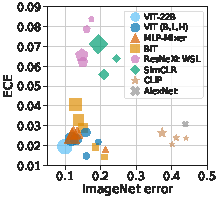
\includegraphics[width=0.35\textwidth]{figs/calibration_plex/vit22b_temperature_scaling_no_ts_no_title.pdf}}\quad\quad 
    \subfigure[Temperature-scaled]{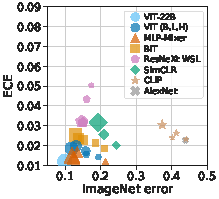
\includegraphics[width=0.35\textwidth]{figs/calibration_plex/vit22b_temperature_scaling_ts_no_title.pdf}}
    \caption{\chonk (light-blue circle) improves the Pareto frontier of the accuracy vs.~the calibration (ECE). Left/right panels are without/with temperature scaling, respectively.}
    \label{fig:calibration}
% \vspace{-10pt}
\end{figure}


\subsubsection{Distillation}
We perform model distillation~\citep{hinton2015distilling} to compress the \chonk into smaller, more widely usable ViTs.
We distill \chonk into ViT-B/16 and ViT-L/16 by following the procedure of~\citet{beyer2022knowledge}.
Using ImageNet-finetuned (at 384px) \chonk, we annotated 500 random augmentations and mixup transforms of each ImageNet image with \chonk logits.
Then, we minimize the KL divergence between the student and the teacher predictive distributions.
We train for 1000 epochs after initializing the student architecture from checkpoints pre-trained on JFT.
The results are shown in \cref{tab:distillation_imagenet}, and we see that we achieve new SOTA on both the ViT-B and ViT-L sizes.
% Appendix \todo{XYZ} contains further details.

\begin{table}[tbp]
%\vspace{-5pt}
    \caption{
      %\textbf
      Distillation results, finetuned at 384 resolution.
}
\centering
  \setlength{\tabcolsep}{4pt}
  \resizebox{0.6\textwidth}{!}{%
    \begin{tabular}{@{} l l c @{}}
      \toprule
	    Model      & &
	    ImageNet1k %Test 
	    \\
      \midrule
      \multirow[c]{4}{*}{\rotatebox{90}{ViT-B/16}}
    %   ViT-B/16~\citep{touvron2022deit} (scratch) & 85.0 \\
    %   ViT-B/16 distilled from \chonk (scratch) & \textbf{?} \\      
      %ViT-B/16
      &~\citep{dosovitskiy2020image} (JFT ckpt.) & 84.2 \\
      %ViT-B/16
      &~\citep{zhai2022scaling} (JFT ckpt.) & 86.6 \\
      %ViT-B/16
      &~\citep{touvron2022deit} (INet21k ckpt.) & 86.7 \\
      %ViT-B/16
      & Distilled from \chonk (JFT ckpt.) & \textbf{88.6} \\
      \midrule
    %   ViT-L/16~\citep{touvron2022deit} (scratch) & 85.8 \\
    %   ViT-L/16 distilled from \chonk (scratch) & \textbf{?} \\   
          \multirow[c]{4}{*}{\rotatebox{90}{ViT-L/16}}
      %ViT-L/16 
      &~\citep{dosovitskiy2020image} (JFT ckpt.) & 87.1 \\
      %ViT-L/16 
      &~\citep{zhai2022scaling} (JFT ckpt.) & 88.5 \\
      %ViT-L/16 
      &~\citep{touvron2022deit} (INet21k ckpt.) & 87.7 \\
      %ViT-L/16 
      & Distilled from \chonk (JFT ckpt.) & \textbf{89.6} \\ 
      \bottomrule
 \end{tabular}
 }
    \label{tab:distillation_imagenet}
    % \vspace{-10pt}
\end{table}


